\documentclass[journal]{IEEEtran}
\usepackage{blindtext}
\usepackage{graphicx}
\usepackage[english]{babel}
\usepackage{pinyin}
\usepackage{natbib}
\usepackage{notoccite}
\usepackage{amssymb}
\usepackage{textcomp}
\usepackage{floatrow}
\usepackage{amsmath}
%
\begin{document}
%
% paper title
\title{Real-Time Application of Activity Classification from Body-Worn Accelerometers}
%
\author{Craig~Euler, C.T. Lin, Melissa Flores, et al? (Ruben, Bryan, Sydney, Steve?)}
%
% make the title area
\maketitle
%
\begin{abstract}
Body worn sensors have been used in the market for many years now.
Many of which are used for activity monitoring or fitness.
In this paper, we make use of a matched-filtering algorithm for real-time activity classification from data obtained with three-axis accelerometers worn by the user.
We achieve invariance to sensor orientation with dimensionality reduction.
We make use of an instance-based learning algorithm to train the device to learn the individual's motion patterns and store that information as activity filters for our matched filter.
We improve computational efficiency with dimensionality reduction, temporal decomposition, and pre-processing of our filters for later use.
An assessment of our computational costs are provided as processing flop counts for the real-time specific parts of the algorithms.
\end{abstract}
%
\section{Introduction}
Various methods for activity classification exist.
Custom dicision tree, automatically generated decision tree, and artificial neural networks \cite{parkka_ermes_korpipaa_mantyjarvi_peltola_korhonen_2006} have been explored as well as other frequency based classification methods \cite{sharma_purwar_lee_lee_chung_2008}.
In this paper, we employ the use of a matched-filter method to identify an individual’s activity in real-time.
The matched-filtering method with use of thresholding and comparing the correlations of various filters is a simple method to use and have been studied in the past \cite{giannakis_tsatsanis_1990}.
Computational resources are limited on micro-processors so we've designed our algorithms to be as efficient as possible.
Having an a priori knowledge of the activity the individual is performing is useful for many current fitness algorithms.
These devices (Fit-Bit, Apple watch, Moov, Jawbone, etc.) usually have the individual input the activity they are performing.
%
\section{Activity Classification via Matched Filtering}
The matched-filter method is commonly used for extracting a signal out of noisy data.
We employ this method for identifying a user’s activity from data generated by body-worn accelerometers.
Because the matched-filter method requires use of an existing reference template to identify the desired signal, we must develop our template from a training set.
We will discuss how we develop our set of templates for use in our matched-filter.

The matched filter is based on the cross correlation of the data $\vec{y} = \{y\}_{k=0}^{N-1}$ with the reference signal $\vec{x} = \{x\}_{k=0}^{M-1}$.
% put this later when we refer to the convolution theorem
If we define $\vec{x}'$ to be $\vec{x}$ that has been zero padded to the length of $\vec{y}$ with the added restriction that the length of $\vec{x}$ be no more than half the length of $\vec{y}$ for preventing corruption with circular indexing, then the cross correlation of $\vec{x}$ with $\vec{y}$ is defined as:
%
\begin{equation} \label{cross_correlation_eq}
(\vec{x} \star \vec{y}) = \{\sum_{i=0}^{M}(x_{i} y_{(i+k)\%N})\}_{k=0}^{N-M}
\end{equation}
%
which is simply a moving dot product. Here we use $(i+k)\%N$ to represent $i+k$ modulo $N$.
We can then normalize \eqref{cross_correlation_eq} by the following:
%
\begin{equation} \label{norm_cross_correlation_eq}
\widehat{(\vec{x} \star \vec{y})}_k = \frac{(\vec{x} \star \vec{y})_k}{\sqrt{||\vec{x}|| \sum_{p=0}^M y_{p+k}^2}}
\end{equation}
%
where \eqref{norm_cross_correlation_eq} is now bound by $[-1,1]$ and has removed any biased toward high energy.
We are most interested where our reference best matches our data. The resulting max correlation yeilds our matched-filter output:
%
\begin{equation} \label{matched_filter_eq}
MF := \underset{k \in [0, M-N]}{max} \{\widehat{(\vec{x} \star \vec{y})}_k\}
\end{equation}
%
\section{Dimensionality Reduction}
We manage to reduce our computational resources and remove our dependence on sensor orientation at the same time through a process of dimensionality reduction.
We assume that over a short period of time a user’s limb movement is constrained mostly to a two-dimensional plane.
By identifying the plane of motion, we then project the acceleration data onto this plane and re-define our $x$ and $y$ axis accordingly.
By this assumption, activities that are mostly confined to two dimensions will improve our signal identification.

If we let $\{\vec{a}_i\}_{i=0}^{N}$ represent our demeaned acceleration data over some time window $T$ in $\mathbb{R}^3$ then the covariance matrix of our acceleration data is represented by the real-symmetric $3x3$ matrix $Q = \vec{a} \vec{a}^T$.
The resulting eigen vectors of this matrix are orthogonal and point in the directions where the data varies most [cite from some text book here].
By projecting our data on the plain defined by the two most dominant eigen vectors, we've effectively reduced our representation of our data to two dimensions.
%
\section{Training the Module}
We are able to identify an individual\textquotesingle's activity by matching the signal to a reference template.
For our application, we develop a reference signature for our matched filter directly from the person\textquotesingle’s motion signature.
We do this by having the individual perform the specific activity over a specified amount of time and select the sub-interval of time that we find best represents the user's motion signature.
For a given activity, we attempt to find the representative periodic signal s of our individual’s activity to be our template.
%
\section{System Hardware}
The sensor used for this analysis is a three-axis accelerometer unit from Kinetisense.
The unit’s acceleration range is -5g to +5g with a sampling rate of 128Hz.
Samples of walking, sitting, running, and bicycling have been recorded with the device and used for the analysis in this paper.
%
\section{Algorithm Software Structure}
%
The algorithms are broken into three main modules: The training, pre-processing of the data used as references for the matched filtering, and the activity classification itself.

The training module, like the pre-processing module, does not need to be in real time.
This algorithm is the most demanding on computational resources and is rarely ran so this can be performed on a smart phone or tablet.
The purpose of the training module is to derive the reference signal to be used on the micro-controller for real-time processing.
The training process uses the same algorithm kernels as the activity classification.
%
\section{Matched-Filter Performance}
%
To demonstrate how effective the matched-filter is for classification, walking, jogging, and bicycling data has been collected from a single individual. One instance of walking data has been used to train the classifier on and a seperate instance of walking data has been used for comparison. Figure \ref{ROC_walk_to_run_fig} shows the effectiveness of the classifier when comparing walking to jogging and figure \ref{ROC_walk_to_bike_fig} shows the comparison to bicycling. Because the bicycling motions are considerably different from walking relative to jogging, we would expect better performance from for bicycling.
\begin{figure}[!tbp]
\RawFloats
  \centering
     \begin{minipage}[b]{0.45\textwidth}
        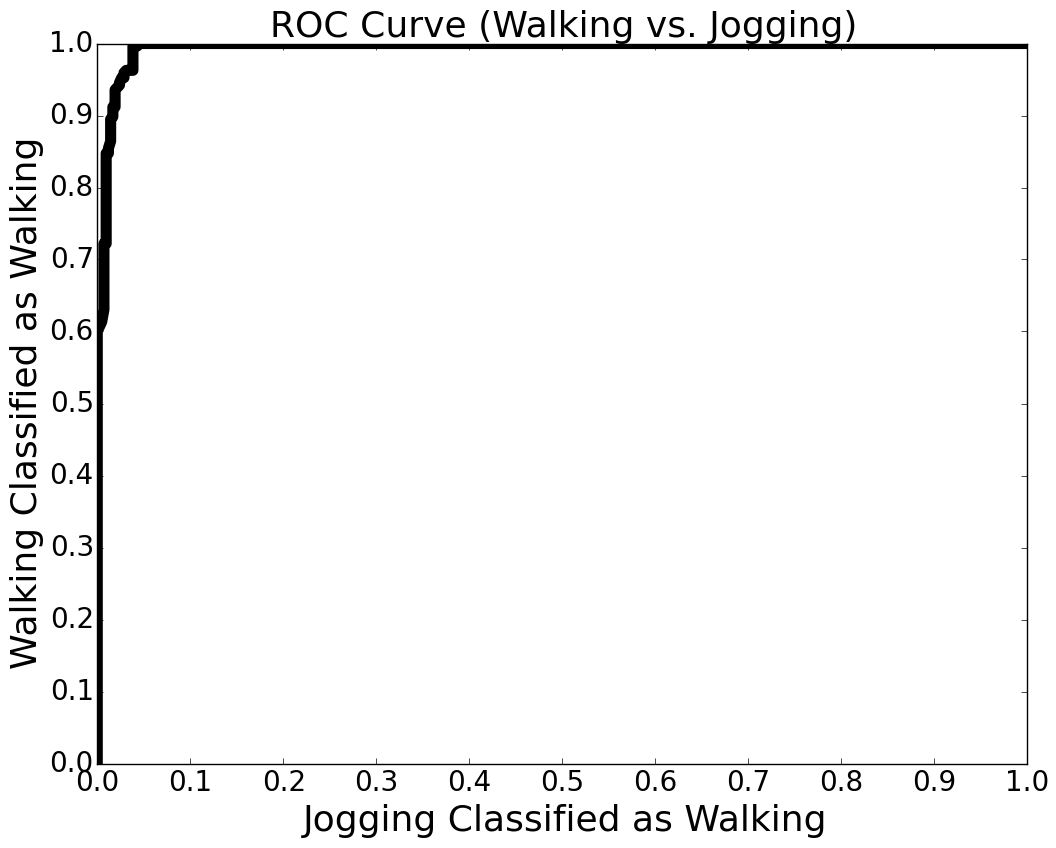
\includegraphics[angle=0,width=\textwidth]{ROC_walk_to_run.png}
        \caption{\label{ROC_walk_to_run_fig}ROC curve with a downsample factor of 8}
     \end{minipage}
     \hfill
     \begin{minipage}[b]{0.45\textwidth}
     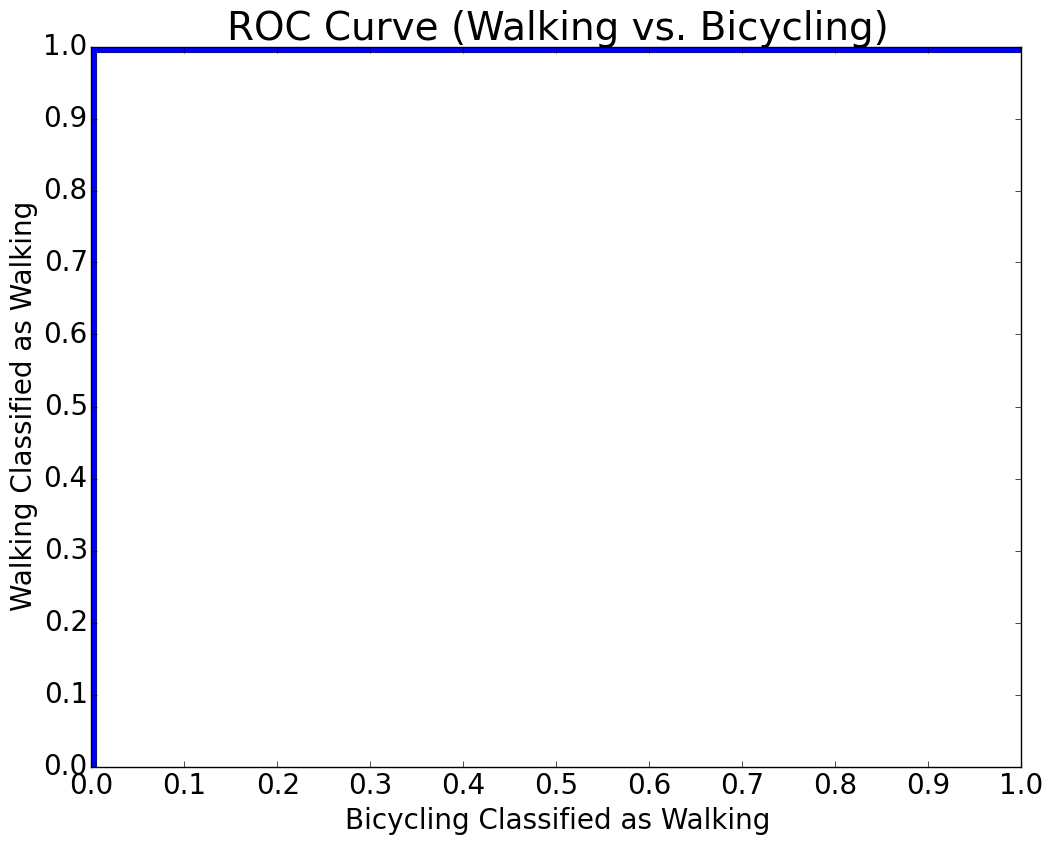
\includegraphics[angle=0,width=\textwidth]{ROC_walk_to_bike.png}
        \caption{\label{ROC_walk_to_bike_fig}ROC curve with a downsample factor of 8}
     \end{minipage}
\end{figure}
%\FloatBarrier
reference to figure \ref{ROC_walk_to_run_fig}
%
\section{Conclusion}
conclusion text.
%
\appendices
%
\ifCLASSOPTIONcaptionsoff
  \newpage
\fi
%
\bibliographystyle{plain}
\bibliography{reference}
\end{document}
